\documentclass{article}
\usepackage{fullpage}
\usepackage{float}
\usepackage{graphicx}

\title{MAESTRO: MAchine and Environment\\Software Translation to ROs}
\author{Christopher T.~Cannon and Jeffrey Segall}
\begin{document}
\maketitle

\section{Introduction}
This document describes the MAchine and Environment Software Translation
to ROs (MAESTRO) software. This includes background information on the
project, system architecture, and installation/running. The purpose of
MAESTRO is to provide an environment to operate the HUBO++ robot both on
the HUBO++ hardware and in a simulation environment.

\section{Background}
The project is funded by the National Science Foundation to work with
the HUBO++ robot. The software is based on Conductor, a software
framework designed to work with the previous HUBO model Jaemi.
The MAESTRO software currently relies upon three other software
components: (1) Orocos, (2) ROS and (3) OpenRAVE.

Orocos is a real-time toolkit to provide hard real-time communication.
The previous Conductor software also relied upon this toolkit as well
and we feel that it is the best open source tool which operates in a
Linux environment. 

The Robot Operating System (ROS) is an open source set of libraries and
tools to help software developers create robot applications. ROS
provides hardware abstraction, device drivers, libraries, visualizers,
message-passing, package management, and other functionality. We
incorporated ROS into the MAESTRO software so that other components
could easily communicate over its message passing interface.

OpenRAVE is an open source simulation environment for testing,
developing, and deploying motion planning algorithms in real-world
robotics applications. OpenRAVE focuses on simulation and analysis of
kinematic and geometric information related to motion planning. MAESTRO
currently only supports OpenRAVE as a simulation environment. However,
we do plan to incorporate other simulation environments (\emph{e.g.},
SimLab).

\section{MAESTRO Architecture}
This section described the MAESTRO architecture and how some of the
source files included in the distribution tie into the operation of the software.

The MAESTRO architecture, shown in Figure~\ref{fig:maestro-arch},
depicts the main components of the system. First is the MAESTRO
component, its main class located in \texttt{maestro/src/HuboCtrl.cpp},
is written in C++ to interact with Orocos and is the interface for all
live hardware or simulation interactions. It utilizes the Orocos
real-time toolkit to ensure hard real-time communication. When
communicating to the live HUBO++ hardware the MAESTRO software
communicates through Orocos and outputs CAN packets on the CAN bus.
These CAN packets signal the physical motors to fire on the HUBO++
robot.

\begin{figure}[H]
    \centering
    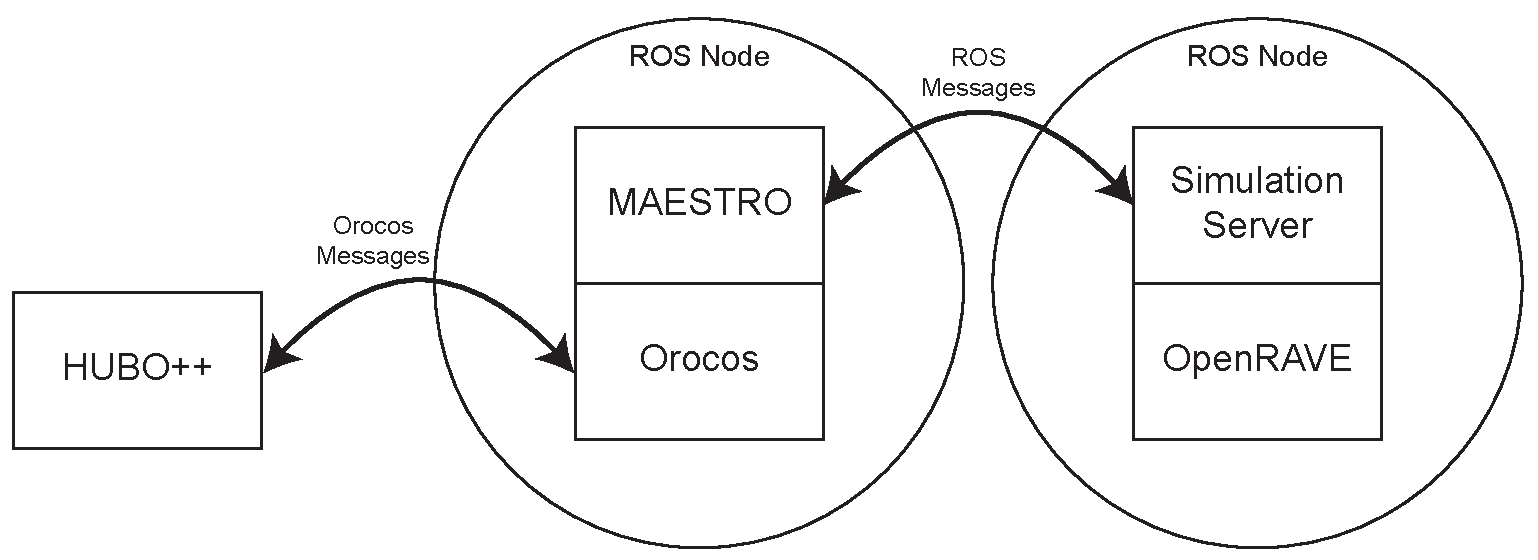
\includegraphics[width=4in]{./art/maestro-architecture.pdf}
    \label{fig:maestro-arch}
    \caption{MAESTRO architecture.}
\end{figure}

When communicating with a simulation environment (at this moment that
can only be OpenRAVE) the MAESTRO software utilizes the ROS
communication bus to pass ROS messages to another ROS node which
contains the OpenRAVE simulation server. The OpenRAVE simulation server,
written in Python and located in \texttt{maestro/src/maestro.py},
initializes and controls the OpenRAVE simulation environment with the
Jaemi HUBO model. Essentially the simulation server listens on a ROS topic for
control messages and moves the specified joint to the specified angle in
the simulator. The OpenRAVE component is merely the GUI which displays
the simulator to the user.

\section{Using MAESTRO}
This section describes how to install and run MAESTRO.

\subsection{Installation}
To install MAESTRO execute the following steps:
\begin{enumerate}
    \item Clone the git repository: \texttt{git clone git@github.com:chriscannon/maestro.git}
    \item Change into the MAESTRO directory: \texttt{cd maestro}
    \item Run the install script as root: \texttt{sudo ./install.sh}
    \item Edit \texttt{/opt/ros/diamondback/setup.sh} to include the
        current location of the MAESTRO code under the
        ROS\_PACKAGE\_PATH variable
\end{enumerate}
Depending on the system, the install can take between 20-to-30 minutes
as the entire ROS and Orocos framework have to be installed and the
OpenRAVE plugin compiled from source.

\subsection{Running}
To run MAESTRO execute the run script \texttt{./run.sh}. This will
launch Orocos and the OpenRAVE GUI to display the simulated HUBO robot.

\end{document}
